\documentclass[12pt]{report}
\usepackage{graphicx}
\usepackage[utf8]{inputenc}
\usepackage[spanish]{babel}
\usepackage{setspace}
\usepackage{geometry}
\usepackage{titlesec}
\usepackage{times}
\usepackage{mathptmx} % Use mathptmx instead of times
\usepackage{fancyhdr}
\usepackage{float}



% Configuración de márgenes
\geometry{
    top=2.5cm,
    left=3cm,
    right=3cm,
    bottom=2.5cm
}

% Configuración de interlineado
\onehalfspacing

% Configuración de títulos y subtítulos
\titleformat{\chapter}[display]
  {\normalfont\bfseries\centering}{}{0pt}{\fontsize{14}{16}\selectfont}
\titleformat{\section}
  {\normalfont\bfseries}{\thesection}{1em}{\fontsize{12}{14}\selectfont}
\titleformat{\subsection}
  {\normalfont\bfseries}{\thesubsection}{1em}{\fontsize{12}{14}\selectfont}


% Configuración de pie de página
  \fancyhf{}
\fancyfoot[R]{\thepage}
\pagestyle{fancy}
\fancypagestyle{plain}{
  \fancyhf{}
  \fancyfoot[R]{\thepage}
}

  \begin{document}
  \pagenumbering{roman}
%----- PORTADA ----
\setlength{\hoffset}{27 pt} % 1 (Para centrar más la portada)
\begin{titlepage}
{\centering
{\fontfamily{ptm}\scshape\bfseries\fontsize{29.16}{34.992}\selectfont Universidad de Guadalajara \par}
\vspace{0.5cm}
{\scshape\Large Centro Universitario de los Lagos \par}
\vspace{1cm}
{\scshape\Large División de Estudios de la Biodiversidad e innovación Tecnológica \par}
\vspace{1cm}
{\graphicspath{{imagenes/Portada}} %ruta de las imagenes

\includegraphics[width=0.3\textwidth]{image.png}\par}
\vspace{1cm}
% Título
{\scshape\large\bfseries Investigación 1. Tipos de Arquitectura \par}
\vspace{1.5cm}
% Materia
{\large \textbf{Asignatura:} \\Sistemas Embebidos\par}
\vfill
% Estudiante
{\large \textbf{Presenta:} \\Oscar Iván Moreno Gutiérrez \#220942754\par}
\vfill
% Profesor
{\large \textbf{Profesor:} \\Dr. Afanador Delgado Samuel Mardoqueo \par}
\vfill
\vfill
% Fecha
\begin{flushright}
  {\normalsize \textbf {Fecha:} \\ \today}
\end{flushright}
\vfill}
{\large  \par}
\end{titlepage}
%----- FIN DE PORTADA ----

%----- ÍNDICE GENERAL ----
\tableofcontents
\newpage

%----- PALABRAS CLAVE ----
\pagenumbering{arabic}
\chapter*{Palabras Clave}
\addcontentsline{toc}{chapter}{Palabras Clave}
\begin{itemize}
  \item Arquitectura de Computadoras: Es el diseño y estructura de los componentes de una computadora, incluyendo el CPU, la memoria y los periféricos.
  \item RISC: Arquitectura de computadoras que utiliza un conjunto de instrucciones reducido y optimizado para mejorar la eficiencia energética.
  \item CISC: Arquitectura de computadoras que busca minimizar el número de instrucciones por programa, aunque a costa de aumentar el número de ciclos por instrucción.
  \item Von Neumann: Arquitectura de computadoras que utiliza una sola unidad de memoria para almacenar tanto los datos como las instrucciones.
  \item Harvard: Arquitectura de computadoras que utiliza unidades de memoria separadas para almacenar los datos y las instrucciones, lo que permite un acceso más rápido a la información.
  \item Sistemas Embebidos: Son sistemas informáticos diseñados para realizar tareas específicas, generalmente integrados en otros dispositivos o sistemas más grandes.
  \item Pipelining: Técnica utilizada en los procesadores para ejecutar múltiples instrucciones en paralelo, dividiendo el proceso en etapas.
  \item CPU: Unidad Central de Procesamiento, es el componente principal de una computadora que realiza las operaciones y ejecuta las instrucciones.
  \item Memoria: Componente de una computadora que almacena los datos y las instrucciones que el CPU necesita para realizar las operaciones.
  \item Periféricos: Dispositivos conectados a una computadora que permiten la entrada y salida de datos, como teclados, ratones, impresoras, etc.
  \item Sistema Operativo: Software que controla y coordina el funcionamiento de los componentes de una computadora y permite la ejecución de programas.
  \item Eficiencia Energética: Capacidad de un sistema para realizar sus funciones utilizando la menor cantidad de energía posible.
  \item Ciclos por Instrucción: Número de ciclos de reloj necesarios para ejecutar una instrucción en un procesador.
  \item Instrucciones por Programa: Número de instrucciones que componen un programa de computadora.
\end{itemize}
\newpage

%----- OBJETIVO ----
\chapter*{Objetivo}
\addcontentsline{toc}{chapter}{Objetivo}
El objetivo de este documento es investigar y analizar los diferentes tipos de arquitecturas de computadoras, incluyendo RISC, CISC, Von Neumann y Harvard, así como identificar sus características principales y los contextos en los que son comúnmente utilizados.
\newpage

%----- CONTENIDO ----
\chapter{Contenido}
\section{Arquitectura de un Sistema Embebido}
La arquitectura de un sistema embebido está diseñada para optimizar el rendimiento, la fiabilidad y la eficiencia energética para tareas específicas.
\begin{figure}[H]
  \centering
  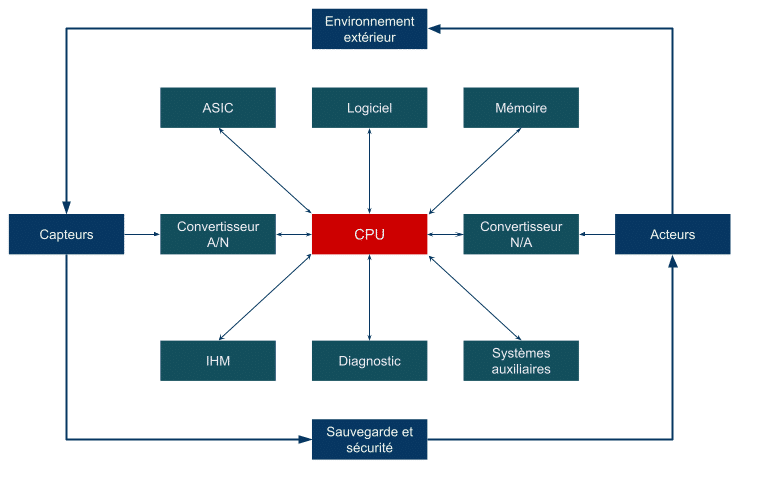
\includegraphics[width=0.5\textwidth]{image2.png}
  \caption{Diagrama de un sistema embebido general.}
  \label{fig:risc}
\end{figure}
Un sistema embebido típico consta de un CPU, memoria, periféricos, y un sistema operativo. \cite{2}
\section{Tipos de Arquitectura}
\subsection{RISC}
La arquitectura de hardware puede implementarse para ser específica de hardware o específica de software, pero según la aplicación se utilizan ambas en la cantidad requerida.

RISC (Reduced Instruction Set Computer) se utiliza en dispositivos portátiles debido a su eficiencia energética.
Utiliza un conjunto de instrucciones altamente optimizado, reduciendo los ciclos por instrucción a costa del número de instrucciones por programa.
\begin{figure}[H]
  \centering
  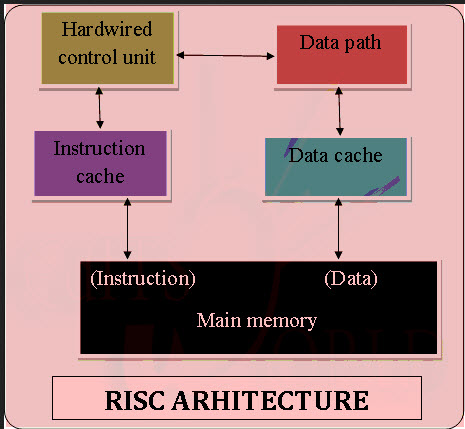
\includegraphics[width=0.5\textwidth]{RISC.png}
  \caption{Arquitectura RISC.}
  \label{fig:risc}
\end{figure}
\subsubsection{Pipeline}
El pipelining (o pipeline) es una característica estándar en los procesadores RISC (Reduced Instruction Set Computer) y funciona de manera similar a una línea de ensamblaje. Permite que el procesador trabaje en diferentes etapas de una instrucción al mismo tiempo, lo que resulta en la ejecución más rápida de múltiples instrucciones.\cite{3}
\subsubsection{Características}
\begin{itemize}
  \item Tiempo de ejecución de un ciclo.
  \item Instrucciones de tamaño fijo.
  \item Instrucciones simples.
  \item Un ciclo por instrucción.
  \item Mayor cantidad de registros.
  \item Mayor cantidad de instrucciones.
\end{itemize}
\subsection{CISC}
El enfoque CISC (Complex Instruction Set Computer) busca minimizar el número de instrucciones por programa, aunque a costa de aumentar el número de ciclos por instrucción. Los ordenadores basados en arquitectura CISC están diseñados para reducir el costo de la memoria. Esto se debe a que los programas grandes requieren más almacenamiento, lo que aumenta el costo de la memoria. Para abordar este problema, se pueden combinar múltiples operaciones en una sola instrucción, lo que hace que las instrucciones sean más complejas pero reduce su cantidad.\cite{1}
\begin{figure}[H]
  \centering
  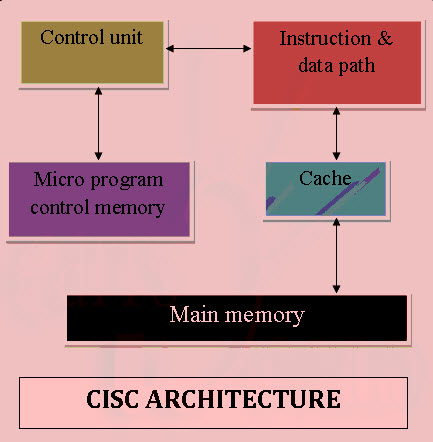
\includegraphics[width=0.5\textwidth]{CISC.png}
  \caption{Arquitectura CISC.}
  \label{fig:cisc}
\end{figure}
\subsubsection{Características}
\begin{itemize}
  \item Lógica de decodificación de instrucciones compleja.
  \item Se requiere una instrucción para soportar múltiples modos de direccionamiento.
  \item Menos espacio en el chip para los registros de propósito general, ya que las instrucciones operan directamente en la memoria.
\end{itemize}

\subsection{Von Neumann}
Una arquitectura de computadora que utiliza una sola unidad de memoria dentro de la cual se almacenan tanto los datos como las instrucciones se conoce como arquitectura de Von Neumann.\cite{4}
\begin{figure}[H]
  \centering
  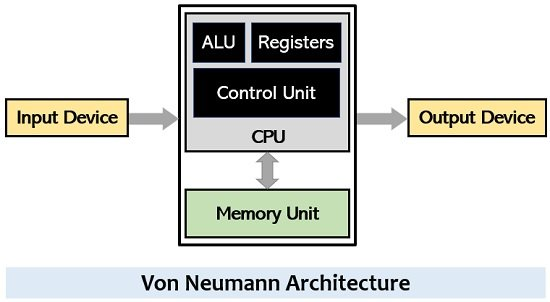
\includegraphics[width=0.5\textwidth]{VonNeuman.png}
  \caption{Arquitectura de Von Neumann.}
  \label{fig:von}
\end{figure}
\subsubsection{Características}
\begin{itemize}
  \item Programa almacenado: Tanto los datos como las instrucciones se guardan en la misma memoria.
  \item CPU: Contiene una unidad aritmético-lógica (ALU) y una unidad de control.
  \item Memoria compartida: Almacena datos e instrucciones.
  \item Almacenamiento masivo externo: Se utiliza para guardar programas y datos a largo plazo.
\end{itemize}
\subsection{Harvard}
Una arquitectura de computadora donde la unidad de memoria se divide en dos partes para almacenar datos e instrucciones individualmente se conoce como arquitectura Harvard. \cite{4}
\begin{figure}[H]
  \centering
  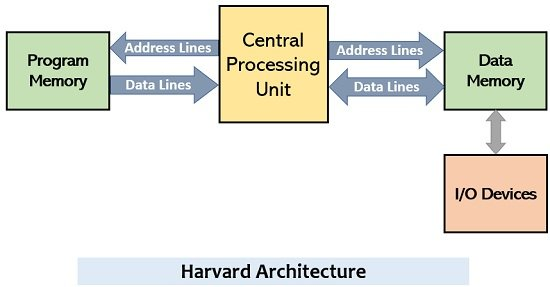
\includegraphics[width=0.5\textwidth]{Harvard.png}
  \caption{Arquitectura de Harvard.}
  \label{fig:harvard}
\end{figure}
\subsubsection{Características}
\begin{itemize}
  \item Memoria separada: Almacena datos e instrucciones en unidades de memoria separadas.
  \item Acceso más rápido: Permite un acceso más rápido a los datos e instrucciones.
  \item Mayor ancho de banda: Permite la transferencia simultánea de datos e instrucciones.
  \item Menor costo: Reduce el costo de la memoria al utilizar unidades de memoria más pequeñas.
\end{itemize}

\section{¿Dónde se utilizan?}
\begin{itemize}
  \item RISC: Dispositivos portátiles, sistemas embebidos, teléfonos móviles, tabletas.
  \item CISC: Computadoras personales, servidores, estaciones de trabajo.
  \item Von Neumann: Computadoras personales, servidores, sistemas embebidos.
  \item Harvard: Sistemas embebidos, microcontroladores, sistemas de control.
\end{itemize}
\newpage

%----- CONCLUSIONES ----
\chapter{Conclusiones}

Se ha investigado y analizado los diferentes tipos de arquitecturas de computadoras, incluyendo RISC, CISC, Von Neumann y Harvard. Se han identificado sus características principales y los contextos en los que son comúnmente utilizados.

Se ha observado que la arquitectura RISC se utiliza en dispositivos portátiles debido a su eficiencia energética. Utiliza un conjunto de instrucciones altamente optimizado, reduciendo los ciclos por instrucción a costa del número de instrucciones por programa. Por otro lado, la arquitectura CISC busca minimizar el número de instrucciones por programa, aunque a costa de aumentar el número de ciclos por instrucción.

La arquitectura de Von Neumann utiliza una sola unidad de memoria para almacenar tanto los datos como las instrucciones. Por otro lado, la arquitectura de Harvard utiliza unidades de memoria separadas para almacenar los datos y las instrucciones, lo que permite un acceso más rápido a la información.

En conclusión, cada tipo de arquitectura tiene sus ventajas y desventajas, y su elección depende del contexto y los requisitos específicos del sistema embebido. Es importante considerar factores como la eficiencia energética, el rendimiento y la complejidad del diseño al seleccionar la arquitectura adecuada para un proyecto de sistemas embebidos.

\newpage
%----- REFERENCIAS ----
\addcontentsline{toc}{chapter}{Bibliografía}
\begin{thebibliography}{1}
\bibitem{1} Arquitectura RISC y CISC: Sus características y ventajas. (2020, diciembre 8). Mefics.org. https://mefics.org/es/qu\%c3\%a9-es-la-arquitectura-risc-y-cisc-con-sus-ventajas-y-desventajas/
\bibitem{2} Daniel. (2024, agosto 2). Los sistemas embebidos: ¿Qué son? ¿Cómo funcionan? Formación en ciencia de datos | Datascientest.com. https://datascientest.com/es/sistemas-embebidos
\bibitem{3} Pipelining. (s/f). Stanford.edu. Recuperado el 22 de agosto de 2024, de https://cs.stanford.edu/people/eroberts/courses/soco/projects/risc/pipelining/index.html
\bibitem{4} Xdc. (2022, marzo 17). Diferencia entre Von Neumann y la arquitectura de Harvard. UNIGAL.MX . https://unigal.mx/diferencia-entre-von-neumann-y-la-arquitectura-de-harvard/




\end{thebibliography}

\end{document}